% =====================================================================
%  Artigo - Projeto Integrador de Teoria dos Grafos - Fase II
%  Estudo de caso: Evacuação e Defesa Civil (Córrego do Feijão, Brumadinho-MG)
%  Formatação: modelo SBC (A4, coluna única, Times 12, margens 3,5/2,5/3,0 cm)
%
%  Conteúdo restrito ao que está no repositório e nas issues da Fase II
%  (#44 a #53, fase2/tabela_lentidao.md, fase2/saida/, README da Fase I).
%  Responsáveis por seção (issue #55):
%    P1 Caroline  -> 3.1 Base de dados e estrutura, 3.2 Modelagem de pesos, 4.1
%    P2 Ian       -> 3.3 Vértice mais próximo e propagação, 4.2 (propagação)
%    P3 Matheus   -> 3.3 Pontes com metadados, 4.2 (vias críticas)
%    P4 Guilherme -> 3.4 Cobertura de Vértices, 3.5 Protocolo experimental
%    P5 Bruno     -> Resumo/Abstract, 1, 2, 5, revisão e formatação final
%
%  Compilação recomendada:  lualatex artigo_fase2.tex   (rodar 2x)
%  Também compila com pdflatex (ex.: Overleaf) - o preâmbulo se adapta.
% =====================================================================
\documentclass[12pt,a4paper]{article}

\usepackage{iftex}
\usepackage[T1]{fontenc}
\usepackage{textcomp}
\usepackage{mathptmx}                   % Times
\usepackage[scaled=.92]{helvet}         % Helvetica (legendas)
\usepackage{courier}
\ifLuaTeX
  \IfFileExists{brazilian.ldf}{%
    \usepackage[brazilian]{babel}%
  }{%
    % Ambiente sem o pacote babel-portuges: usa o .ini do babel e carrega
    % os padrões de hifenização do português (hyph-pt.pat.txt) em tempo real.
    \usepackage[provide=*]{babel}
    \babelprovide[import=pt-BR, main]{brazilian}
    \directlua{
      local f = io.open("hyph-pt.pat.txt")
      if f then
        local p = f:read("*a"); f:close()
        p = p:gsub("\string\n", " ")
        tex.print("\string\\babelpatterns[brazilian]{" .. p .. "}")
      end
    }%
  }
\else
  \usepackage[utf8]{inputenc}
  \usepackage[brazilian]{babel}
\fi

\usepackage[a4paper,top=3.5cm,bottom=2.5cm,left=3cm,right=3cm]{geometry}
\usepackage{graphicx}
\usepackage{amsmath}
\usepackage{booktabs}
\usepackage{array}
\usepackage{enumitem}
\usepackage{microtype}
\usepackage{xcolor}
\usepackage[hidelinks]{hyperref}
\usepackage{url}
\urlstyle{same}

% ---------------- Estilo SBC ----------------
\pagestyle{empty}                       % sem cabeçalho, rodapé e numeração
\setlength{\parindent}{1.27cm}          % recuo dos parágrafos subsequentes
\setlength{\parskip}{6pt}               % 6 pt antes de cada parágrafo
\frenchspacing
\sloppy

\makeatletter
% Seções: negrito 13 pt, alinhadas à esquerda, 12 pt extras antes
\renewcommand\section{\@startsection{section}{1}{\z@}%
  {12pt}{0.1pt}{\normalfont\fontsize{13}{15}\selectfont\bfseries}}
% Subseções: negrito 12 pt
\renewcommand\subsection{\@startsection{subsection}{2}{\z@}%
  {12pt}{0.1pt}{\normalfont\normalsize\bfseries}}
\renewcommand\thesection{\arabic{section}.}
\renewcommand\thesubsection{\arabic{section}.\arabic{subsection}.}
\renewcommand\@seccntformat[1]{\csname the#1\endcsname\ }
\makeatother

% Legendas: Helvetica 10 pt negrito; centralizadas se tiverem uma linha,
% justificadas com recuo de 0,8 cm caso contrário; 6 pt antes e depois.
\usepackage[font={sf,bf,footnotesize},labelsep=period,justification=justified,
            singlelinecheck=true,margin=0.8cm,skip=6pt]{caption}
\captionsetup[table]{position=top}
\setlength{\abovecaptionskip}{6pt}
\setlength{\belowcaptionskip}{6pt}
\addto\captionsbrazilian{\renewcommand{\tablename}{Tabela}\renewcommand{\figurename}{Figura}}

% Resumo / Abstract: Times 12, recuo de 0,8 cm nas duas margens
\newenvironment{sbcabstract}[1]%
  {\list{}{\leftmargin=0.8cm\rightmargin=0.8cm\topsep=0pt\parsep=0pt}\item[]\textbf{#1.}\ }%
  {\endlist}

% Referências: 12 pt, 6 pt antes de cada uma, recuo de 0,5 cm nas linhas seguintes
\newenvironment{referencias}%
  {\section*{Referências}\begin{list}{}{\leftmargin=0.5cm\itemindent=-0.5cm%
   \labelwidth=0pt\labelsep=0pt\itemsep=0pt\parsep=0pt\topsep=0pt}\setlength{\parskip}{6pt}}%
  {\end{list}}
\newcommand{\referencia}{\item\relax}

\newcommand{\us}{\,\textmu s}


% =====================================================================
\begin{document}
% SBC: o primeiro parágrafo de cada seção não tem recuo (o babel em português o ativaria)
\makeatletter\let\@afterindenttrue\@afterindentfalse\makeatother

\begin{center}
  \vspace*{12pt}
  {\fontsize{16}{19}\selectfont\bfseries
   Pesos, Vias Críticas e Postos de Socorro na Malha Viária de Córrego do Feijão (Brumadinho--MG): Fase II\par}
  \vspace{12pt}
  {\bfseries Caroline Lopes Martins, Ian Melo Gonçalves, Matheus Filipe da Silva Ponte, Guilherme Amaro de Castro, Bruno Nobrega Souza\par}
  \vspace{12pt}
  Curso de Ciência da Computação -- Centro Universitário IESB, Campus Asa Sul\\ Brasília -- DF -- Brasil\par
\end{center}

\begin{sbcabstract}{Abstract}
This paper extends the graph model of the road network around the Córrego do Feijão mine (Brumadinho, Brazil), site of the 2019 B1 dam collapse (3,143 vertices, 3,199 edges), with edge weights that combine Haversine distance and a slowness factor per road type. With these weights the 88.3\,km network behaves as 207.0\,km of reference road, since 61.8\% of it is service roads, rural tracks and footpaths. The paper also describes the tailings propagation from the dam, the bridge edges reported with road metadata, a connected subgraph generator for stress tests and an exact backtracking solver for minimum vertex cover, used to place relief posts.
\end{sbcabstract}

\begin{sbcabstract}{Resumo}
Este artigo estende o modelo em grafo da malha viária do entorno da mina Córrego do Feijão (Brumadinho--MG), onde a barragem B1 se rompeu em 2019 (3.143 vértices e 3.199 arestas), com pesos que combinam a distância de Haversine e um fator de lentidão por tipo de via. Com eles, os 88,3\,km de vias equivalem a 207,0\,km de via de referência, pois 61,8\% da malha são acessos, estradas rurais e trilhas. O artigo descreve ainda a propagação dos rejeitos a partir da barragem, o relatório de pontes com os dados de cada via, um gerador de subgrafos conexos para testes de estresse e uma solução exata por \emph{backtracking} da Cobertura de Vértices, usada para posicionar postos de socorro.
\end{sbcabstract}

% ---------------------------------------------------------------------
\section{Introdução}

Em 25 de janeiro de 2019, a barragem B1 da mina Córrego do Feijão, em Brumadinho (MG), rompeu-se e liberou mais de 11 milhões de m$^3$ de rejeitos, que deixaram 259 mortos e 11 desaparecidos até janeiro de 2020 [Rotta et al. 2020]. A legislação posterior passou a exigir a delimitação da Zona de Autossalvamento, em que a população precisa deixar a área por conta própria [Brasil 2020]. Na Fase I deste projeto, a malha viária da região foi modelada como um grafo não ponderado e analisada quanto à topologia: metade das arestas são pontes, 145 de 351 trechos viários não têm rota alternativa e 107 cruzamentos são pontos únicos de falha.

A topologia indica \emph{se} é possível sair de um ponto, mas não \emph{quanto custa} sair. Uma trilha e uma estrada asfaltada de mesmo comprimento são equivalentes num grafo não ponderado, embora a segunda seja percorrida várias vezes mais rápido. A Fase II atribui a cada via um peso que traduz esse custo e prepara o grafo para duas perguntas da Defesa Civil: \emph{qual a rota mais rápida até um ponto seguro?} (menor caminho, problema da classe P) e \emph{qual o menor número de postos de socorro tal que toda via tenha um posto numa das extremidades?} (Cobertura de Vértices, NP-difícil).

As contribuições são: (i) um modelo de pesos baseado em dados abertos e na legislação de trânsito; (ii) a implementação autoral em C dos módulos de tipo de via, distância, localização de pontos no grafo, propagação dos rejeitos, relatório de pontes, geração de subgrafos e Cobertura de Vértices exata; e (iii) a quantificação do efeito dos pesos sobre a malha da região. As Seções~2 a 5 apresentam, respectivamente, os trabalhos relacionados, a metodologia, os resultados e a conclusão.

% ---------------------------------------------------------------------
\section{Trabalhos Relacionados}

Modelos de evacuação em redes tratam a malha viária como um grafo com custos ou capacidades nas arestas e buscam rotas ou fluxos que minimizem o tempo de saída [Hamacher and Tjandra 2002]. A escolha do custo é decisiva: a biblioteca OSMnx [Boeing 2017], por exemplo, estima o tempo de percurso de cada aresta a partir do comprimento e de uma velocidade associada ao tipo de via do OpenStreetMap, abordagem semelhante à adotada aqui. Com custos não negativos, o menor caminho é obtido pelo algoritmo de Dijkstra [Dijkstra 1959].

A Cobertura de Vértices está entre os 21 problemas que Karp [Karp 1972] provou serem NP-completos em sua versão de decisão; a versão de otimização é, portanto, NP-difícil [Garey and Johnson 1979]. Soluções exatas exigem tempo exponencial no pior caso, enquanto o algoritmo que toma as duas extremidades de cada aresta de um emparelhamento maximal garante uma cobertura no máximo duas vezes maior que a ótima [Cormen et al. 2009]. A localização de serviços de emergência como problema de cobertura remonta a Toregas et al. [Toregas et al. 1971], que buscaram o menor número de instalações capaz de atender todos os pontos de demanda dentro de um tempo máximo; a Cobertura de Vértices é uma versão em grafo dessa ideia, em que o atendimento é a adjacência a um posto.

% ---------------------------------------------------------------------
\section{Metodologia e Modelagem}

\subsection{Base de dados e estrutura}

O dataset é o mesmo da Fase I: 224 vias extraídas do OpenStreetMap [OpenStreetMap contributors 2026], que geram um grafo não direcionado com $|V| = 3.143$ vértices, $|E| = 3.199$ arestas e 88,3\,km de extensão. A estrutura da Fase I foi estendida para guardar, em cada nó da lista de adjacência, o tipo da via (\texttt{highway}) e uma referência aos metadados da via de origem (identificador OSM, nome e nome oficial); um programa de teste confere que todas as 3.199 arestas recebem um tipo. A Fase II usa a lista de adjacência, representação que a Fase I mostrou ser a adequada para esta malha esparsa: no grafo completo, ela ocupa 124,5\,KiB, contra 37,7\,MiB da matriz.

\subsection{Modelagem de pesos}

O peso de uma aresta $(u,v)$ representa o custo de percorrê-la e é definido como
\begin{equation}
w(u,v) = d_H(u,v)\cdot f\big(\mathrm{tipo}(u,v)\big),
\label{eq:peso}
\end{equation}
em que $d_H$ é a distância entre as extremidades pela fórmula de Haversine [Sinnott 1984], com raio terrestre de 6.371\,km, e $f$ é o fator de lentidão do tipo da via. O fator é a razão entre uma velocidade de referência de 40\,km/h e a velocidade assumida para o tipo, de modo que $d_H \cdot f$ equivale a metros percorridos na via de referência.

As velocidades das vias pavimentadas seguem os limites do art.~61 do Código de Trânsito Brasileiro para vias locais (30\,km/h) e coletoras (40\,km/h) [Brasil 1997], associados aos tipos do OpenStreetMap conforme a função de cada um na classificação da plataforma [OpenStreetMap Wiki 2026]. Para acessos, estradas rurais e trilhas, as velocidades são hipóteses do grupo para um cenário de emergência, com chão irregular, possível lama e trechos estreitos (Tabela~\ref{tab:lentidao}). Trilhas recebem fator alto, mas finito: continuam disponíveis para a fuga a pé e são evitadas pelas rotas de veículos sempre que houver alternativa. A capacidade das vias não foi modelada, porque o OpenStreetMap não traz esse dado de forma confiável para a região.

\begin{table}[!htb]
\caption{Fator de lentidão por tipo de via e seu efeito na malha de Córrego do Feijão.}
\label{tab:lentidao}
\centering\small
\begin{tabular}{@{}lrrrrr@{}}
\toprule
\textbf{Tipo (OSM)} & \textbf{Vel. (km/h)} & \textbf{Fator} & \textbf{Arestas} & \textbf{km} & \textbf{km equiv.}\\
\midrule
tertiary              & 40 & 1,00 & 521 & 11,4 & 11,4\\
unclassified          & 30 & 1,33 & 811 & 19,2 & 25,5\\
residential           & 30 & 1,33 & 101 &  3,2 &  4,2\\
tertiary\_link        & 30 & 1,33 &   1 &  0,0 &  0,0\\
service               & 20 & 2,00 & 818 & 24,7 & 49,4\\
track                 & 15 & 2,67 & 726 & 23,0 & 61,4\\
path                  &  5 & 8,00 & 190 &  6,3 & 50,6\\
footway               &  5 & 8,00 &  31 &  0,6 &  4,5\\
\midrule
\textbf{Total}        &    &      & 3.199 & 88,3 & 207,0\\
\bottomrule
\end{tabular}
\end{table}

\subsection{Pontos de referência e análises de apoio}

Pontos do mundo real são associados ao grafo pelo vértice mais próximo de sua coordenada, encontrado por busca linear com a distância de Haversine em $O(|V|)$. A barragem B1 (20,1197\textdegree\,S; 44,1214\textdegree\,W) é associada dessa forma e serve de origem para a propagação dos rejeitos e para os subgrafos de teste.

A propagação da frente de rejeitos é simulada por camadas de uma busca em largura a partir do vértice da B1: a camada de cada vértice representa o tempo relativo de chegada da lama, e o resultado é gravado em \texttt{saida/afetados.csv}. As arestas-ponte, calculadas pelo algoritmo de Tarjan [Tarjan 1972] na Fase I, passaram a ser relatadas com os metadados da via (nome, nome oficial, referência, identificador OSM e tipo), em \texttt{saida/ponte.csv} e \texttt{saida/relatorio\_pontes.txt}, para que a Defesa Civil identifique cada trecho crítico no mapa e em campo.

\subsection{Otimização NP-difícil: Cobertura de Vértices}

Uma cobertura de vértices é um conjunto $C \subseteq V$ tal que toda aresta tem ao menos uma extremidade em $C$. Interpretando cada vértice como um local possível de posto de socorro, uma cobertura mínima é o menor conjunto de postos que deixa toda via com um posto em uma de suas pontas. Como consequência, todo cruzamento que não recebe posto tem todos os vizinhos em $C$ e fica, portanto, a uma aresta de um posto.

A solução exata implementada copia as arestas do grafo não direcionado uma única vez para um vetor (pares com $u < v$) e percorre os vértices em ordem; para cada um, ramifica em duas decisões, incluí-lo ou não na cobertura, por \emph{backtracking} com poda pelo limite superior (\emph{branch and bound}). Um ramo é podado quando o tamanho da seleção atual já iguala ou supera a melhor cobertura encontrada, e cada nó da árvore de busca verifica se todas as arestas estão cobertas, em $O(|E|)$. No pior caso o custo é $O(2^{|V|}\cdot|E|)$, o que restringe a solução exata a grafos pequenos. Os postos escolhidos são gravados em \texttt{saida/cobertura\_exata.csv}, com o identificador e as coordenadas de cada um.

\subsection{Protocolo experimental}

Para os testes de estresse, um gerador extrai subgrafos conexos induzidos pelos $N$ primeiros vértices de uma busca em largura a partir do vértice da B1, com $N = 100$, $500$ e $1.000$, e os grava em arquivos de texto com a lista de vértices (com coordenadas) e de arestas (com o tipo da via). A busca em largura garante que os $N$ vértices pertençam à mesma componente conexa. Cada módulo tem seu próprio executável e registra o tempo de execução (ms) e a memória (bytes, por alocações rastreadas) num \emph{log} comum (RF03). Todo o código é autoral, em C, sem bibliotecas de grafos (RNF01), e é compilado por um único \texttt{Makefile}.

% ---------------------------------------------------------------------
\section{Resultados e Discussão}

\subsection{Efeito dos pesos na malha}

A Tabela~\ref{tab:lentidao} e a Figura~\ref{fig:pesos} mostram o efeito dos pesos. Apenas 12,9\% da extensão é via de referência (\texttt{tertiary}), e 61,8\% corresponde a acessos, estradas rurais e trilhas (\texttt{service}, \texttt{track}, \texttt{path} e \texttt{footway}). Com os pesos, os 88,3\,km de vias equivalem a 207,0\,km de via de referência, ou seja, a malha efetiva é 2,34 vezes maior que a real. As estradas rurais (\texttt{track}) passam a ser o maior componente do custo, com 61,4\,km equivalentes, e as trilhas, com apenas 6,3\,km reais, equivalem a 50,6\,km. As vias rápidas formam um eixo ao sul e a leste da barragem, enquanto o entorno imediato da B1 é servido quase só por acessos e estradas rurais, justamente a região que precisa ser evacuada primeiro.

\begin{figure}[!htb]
\centering
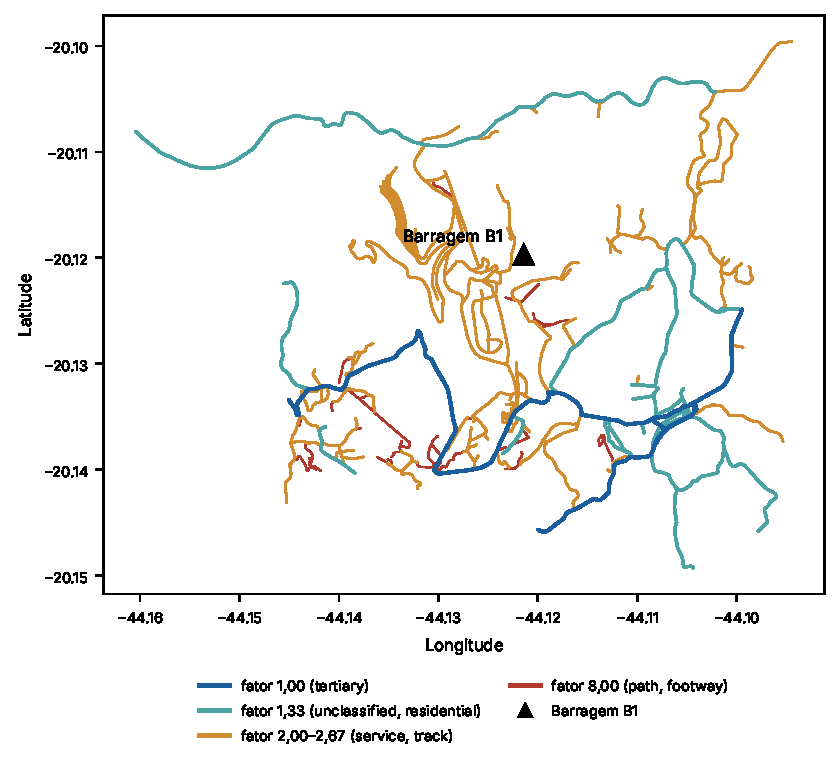
\includegraphics[width=0.80\textwidth]{figuras/mapa_pesos.pdf}
\caption{Malha viária de Córrego do Feijão colorida pelo fator de lentidão do tipo de via. O triângulo marca a barragem B1.}
\label{fig:pesos}
\end{figure}

As velocidades de acessos, estradas rurais e trilhas são hipóteses, não medições, e não houve calibração com dados reais de deslocamento. Como a tabela tem grande influência no custo total, o resultado deve ser lido como uma estimativa da ordem de grandeza da lentidão da malha.

\subsection{Propagação e vias críticas}

A busca em largura a partir do vértice da B1 alcança 3.115 dos 3.143 vértices, até a camada 256; os 28 vértices não alcançados formam os dois fragmentos sem ligação com a rede mapeada identificados na Fase I. Como observado naquela fase, a camada mede segmentos digitalizados e não distância, de modo que a ordem de chegada é útil para priorizar alertas, enquanto o tempo de chegada depende dos pesos da Seção~3.2.

O relatório de pontes com metadados torna as 1.615 arestas-ponte da Fase I acionáveis: cada uma passa a ser identificada pelo nome da via, quando existe, e pelo identificador OSM, o que permite localizá-la em campo. Como a maior parte da malha é formada por acessos e estradas rurais, muitas dessas vias não têm nome no OpenStreetMap, e o identificador OSM é a única referência disponível.

% ---------------------------------------------------------------------
\section{Conclusão e Trabalhos Futuros}

A atribuição de pesos mostrou que a malha de Córrego do Feijão é bem mais lenta do que sua extensão sugere: com o fator de lentidão por tipo de via, os 88,3\,km equivalem a 207,0\,km de via de referência, porque quase dois terços da extensão são acessos, estradas rurais e trilhas, concentrados justamente no entorno da barragem. Os módulos de localização, propagação, pontes com metadados, geração de subgrafos e Cobertura de Vértices exata compõem a base para as etapas de otimização.

Como próximos passos, o grupo definiu: calcular rotas de menor custo com o algoritmo de Dijkstra, gravando a rota em \texttt{saida/rota.csv}; acrescentar ao peso uma componente de risco relativa à origem do desastre; implementar uma heurística gulosa para a Cobertura de Vértices e compará-la à solução exata em tempo e qualidade; e executar os testes de estresse nos subgrafos de 100, 500 e 1.000 vértices. Também se propõe calibrar as velocidades por tipo de via com dados reais de deslocamento e considerar a interdição dos trechos alcançados pela lama ao longo da propagação.

% ---------------------------------------------------------------------
\begin{referencias}
\referencia Boeing, G. (2017). OSMnx: New methods for acquiring, constructing, analyzing, and visualizing complex street networks. \emph{Computers, Environment and Urban Systems}, 65:126--139.

\referencia Brasil (1997). Lei n\textordmasculine{} 9.503, de 23 de setembro de 1997. Institui o Código de Trânsito Brasileiro. \emph{Diário Oficial da União}.

\referencia Brasil (2020). Lei n\textordmasculine{} 14.066, de 30 de setembro de 2020. Altera a Política Nacional de Segurança de Barragens (Lei n\textordmasculine{} 12.334/2010). \emph{Diário Oficial da União}.

\referencia Cormen, T. H., Leiserson, C. E., Rivest, R. L. and Stein, C. (2009). \emph{Introduction to Algorithms}. MIT Press, 3rd edition.

\referencia Dijkstra, E. W. (1959). A note on two problems in connexion with graphs. \emph{Numerische Mathematik}, 1:269--271.

\referencia Garey, M. R. and Johnson, D. S. (1979). \emph{Computers and Intractability: A Guide to the Theory of NP-Completeness}. W. H. Freeman.

\referencia Hamacher, H. W. and Tjandra, S. A. (2002). Mathematical modelling of evacuation problems: a state of the art. In \emph{Pedestrian and Evacuation Dynamics}, pages 227--266. Springer.

\referencia Karp, R. M. (1972). Reducibility among combinatorial problems. In Miller, R. E. and Thatcher, J. W., editors, \emph{Complexity of Computer Computations}, pages 85--103. Plenum Press.

\referencia OpenStreetMap contributors (2026). Dados extraídos via overpass-turbo em 8 set. 2026 (licença ODbL). \url{https://www.openstreetmap.org}.

\referencia OpenStreetMap Wiki (2026). Key:highway. \url{https://wiki.openstreetmap.org/wiki/Key:highway}.

\referencia Rotta, L. H. S. et al. (2020). The 2019 Brumadinho tailings dam collapse: Possible cause and impacts of the worst human and environmental disaster in Brazil. \emph{International Journal of Applied Earth Observation and Geoinformation}, 90:102119.

\referencia Sinnott, R. W. (1984). Virtues of the haversine. \emph{Sky and Telescope}, 68(2):159.

\referencia Tarjan, R. (1972). Depth-first search and linear graph algorithms. \emph{SIAM Journal on Computing}, 1(2):146--160.

\referencia Toregas, C., Swain, R., ReVelle, C. and Bergman, L. (1971). The location of emergency service facilities. \emph{Operations Research}, 19(6):1363--1373.
\end{referencias}

\end{document}
